\chapter{Binäre Bäume}

\section{Lösung}

\begin{itemize}
    \item Im \textbf{worst-case} sind Einfügeoperationen in einem binären Suchbaum von der Komplexitätsklasse $O(n)$
    \item Im \textbf{average-case} sind Einfügeoparationen in einem binären Suchbaum von der Komplexitätsklasse $O(log n)$
\end{itemize}

Im \textbf{}


\begin{figure}
    \begin{center}
        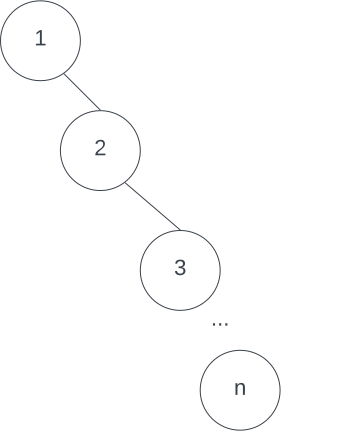
\includegraphics[scale=0.3]{chapters/5. Binäre Bäume/img/degenerate_tree}
        \caption{Für einen entarteten binären Suchbaum sind Einfügeoperationen von der Komplexität $O(n)$ (Quelle: eigene)}
        \label{fig:degeneratetree}
    \end{center}
\end{figure}

\section{Anmerkung und Ergänzungen}

Der \textbf{worst-case} ergibt sich, wenn ein binärer Suchbaum \textbf{entartet} ist - die Reihenfolge der Knoten entspricht dann der Anordnung in einer verketteten List, in der das kleinste Element am Anfang der Liste steht, das größte Element am Ende der Liste.\\
Soll jetzt ein Element eingefügt werden, dessen Schlüssel größer als alle in dem Suchbaum enthaltenen Werte ist, muss der \textit{rechte Teilbaum} bis zum Ende durchwandert werden, um das Element einzufügen.\\
Bei $n$ vorhandenen Knoten ergibt sich somit ein Zeitaufwand von $O(n)$.\\




























